\chapter{Egobets}
\graphicspath{{/Users/brunomedina/Dropbox/Tesis-Egobets/egobets-notas/resources/diagramas/}}

Se describen las cuatro piezas de software desarrolladas que conforman en su totalidad el sistema de Egobets. Las tres primeras permiten al usuario adminstrativo echar a andar toda la maquinaria. Y la última pieza, conocida como el portal público, proporciona al usuario final los servicios del sistema a través de un sitio web usable, práctico y profesional. 
A todo este conjunto de herramientas y programas que el usuario necesita para esta tarea se le conocerá como \emph{Back Office}.

\section{Descripción General}
El ecosistema de Egobets consiste principalmente de cuatro piezas de software. Ver la figura~\ref{Fig:Sistemas}. 




\begin{figure}[!htb]\centering
   \begin {minipage}{1\textwidth}
     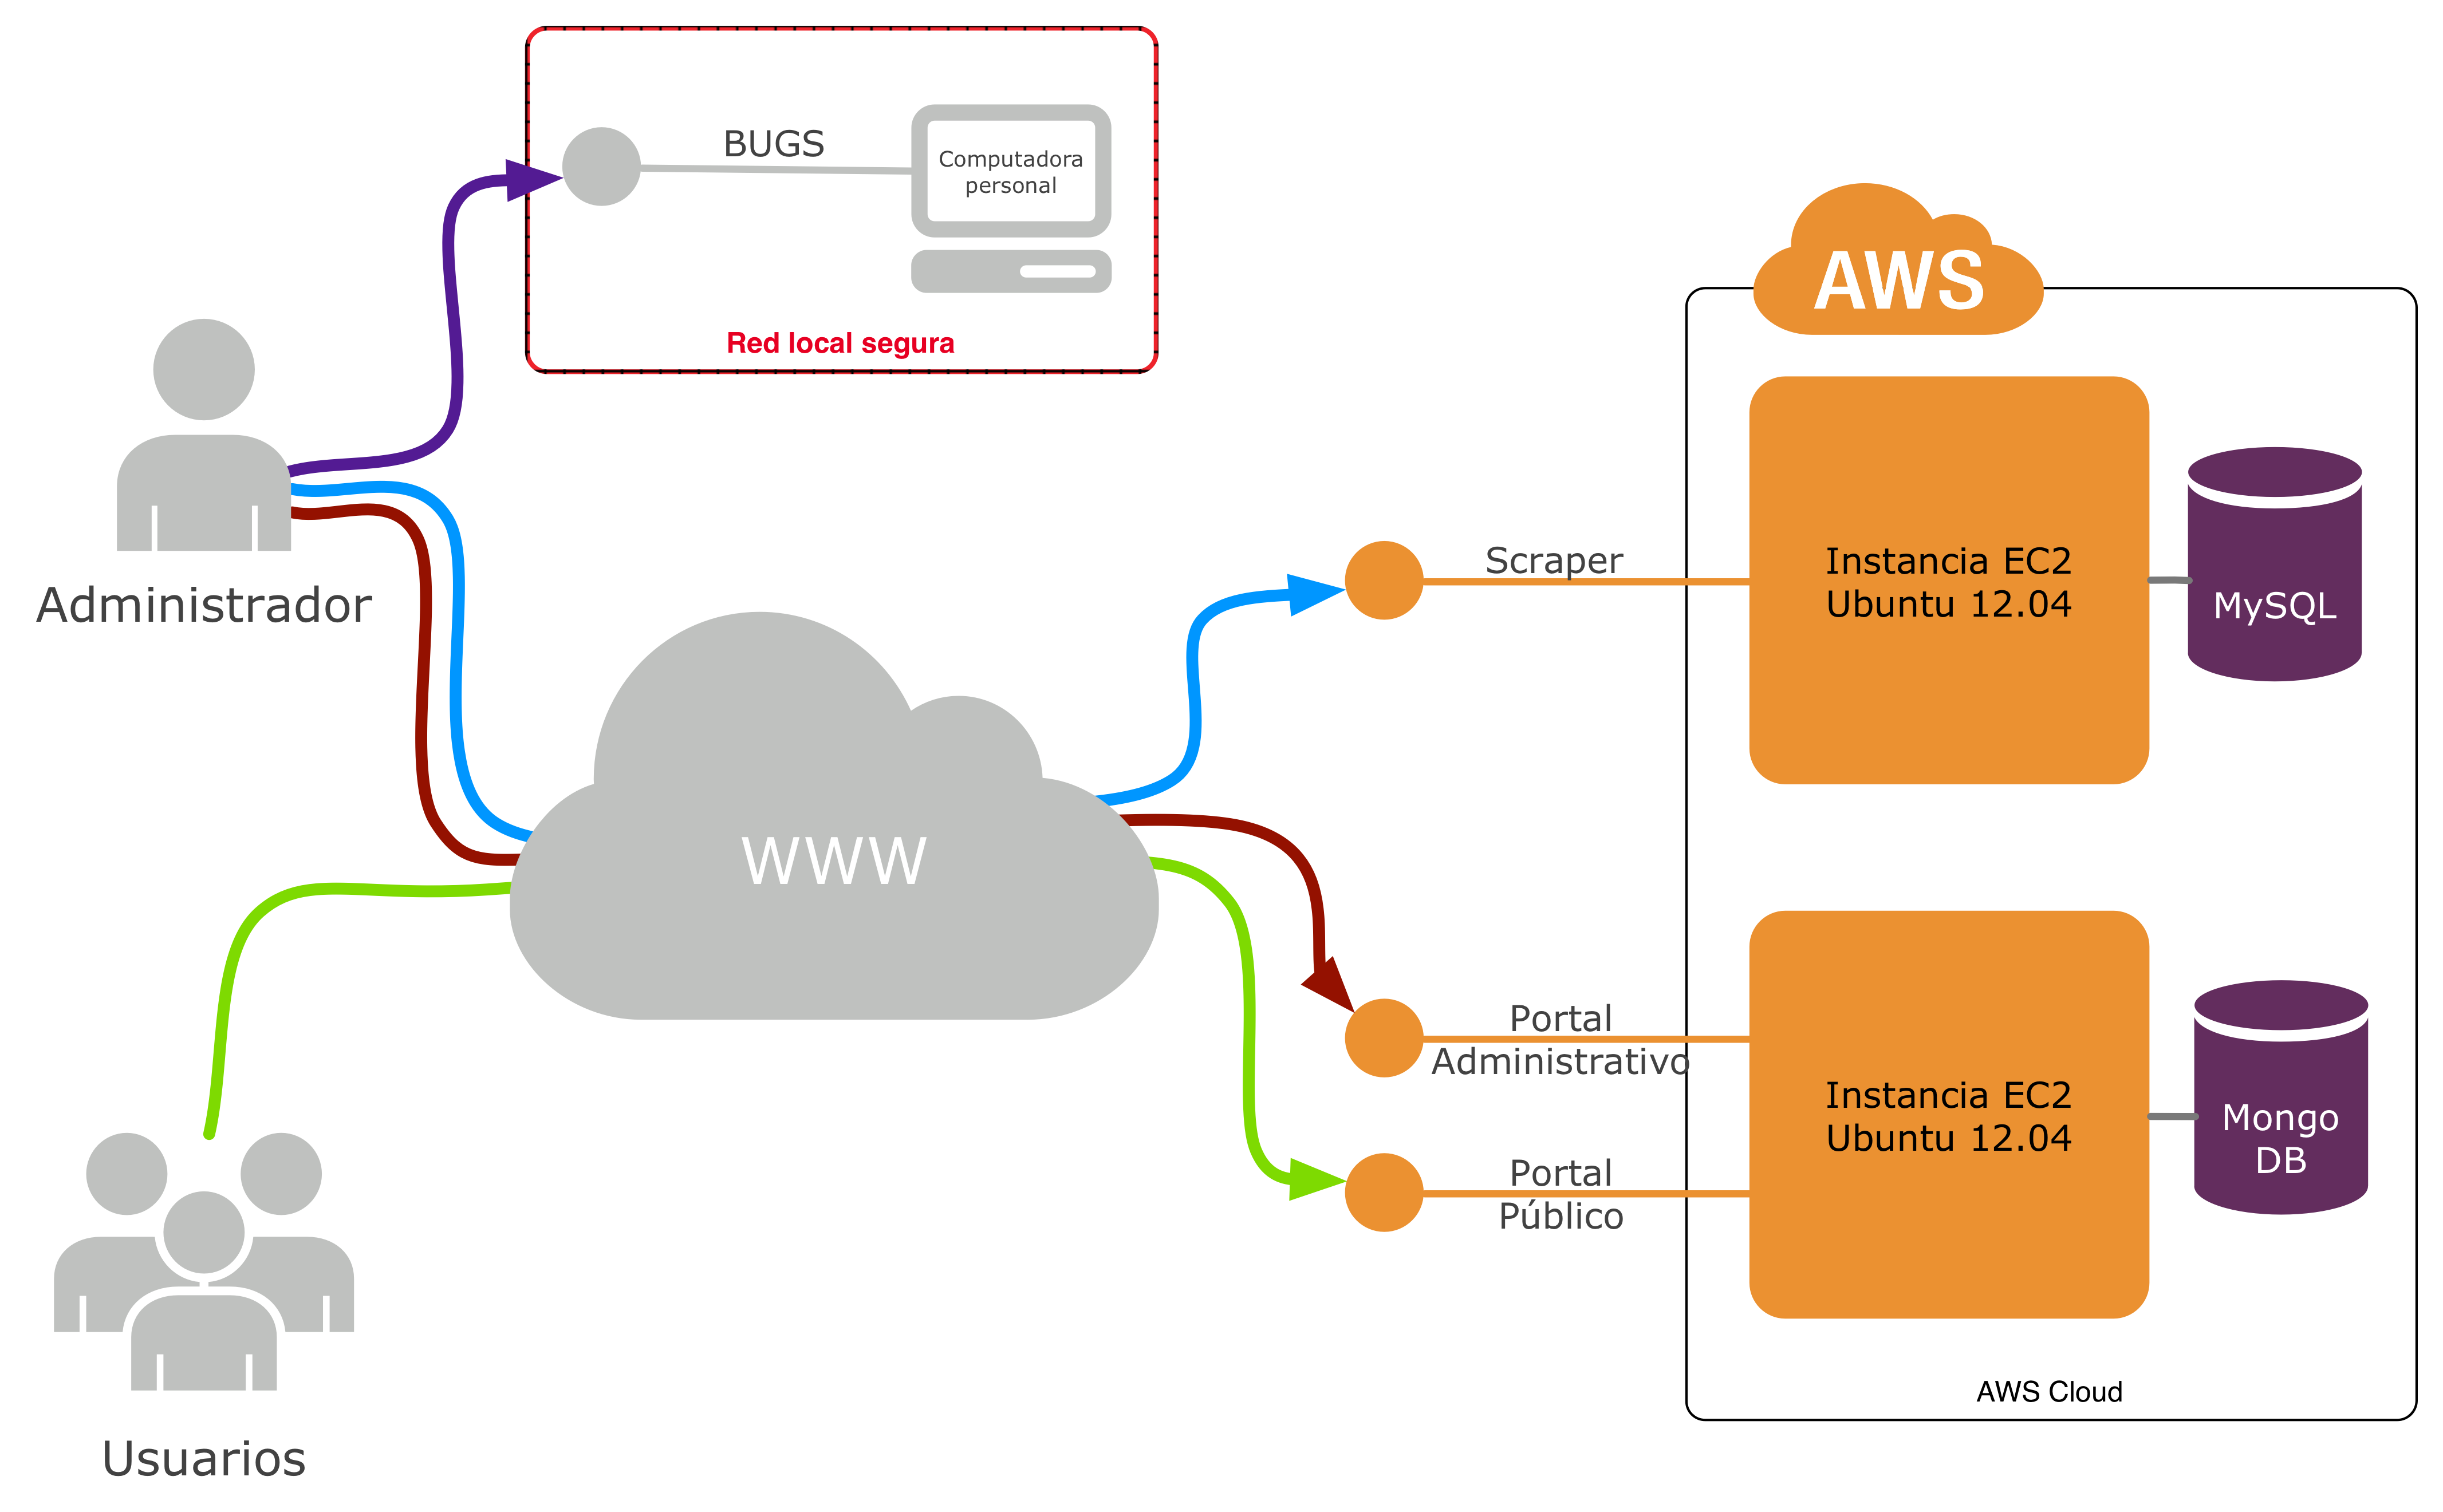
\includegraphics[width=\linewidth]{sistemas}
     \caption{Diagrama de sistemas y usuarios}\label{Fig:Sistemas}
   \end{minipage}
\end{figure}

El Sistema de recopilación de información y estadísiticas de los partidos (\emph{Sistema de recopilación}), el \emph{Portal administrativo} y el \emph{Portal público} corren bajo una arquitectura cliente servidor en la nube de Amazon Web Services; mientras que el Sistema de estimación de probabilidades (\emph{Sistema de estimación}) corre en un ordenador personal.


\subsubsection{Computación en la nube}

El sistema usa la nube para ofrecer sus servicio a los usuarios, se puede decir que el software corre en un esquema tipo ``SaaS''\footnote{Software as a Service. ``Es el más conocido de los niveles de cómputo en la nube. El SaaS es un modelo de distribución de software que proporciona a los clientes el acceso a éste a través de la red (generalmente Internet). De esta forma, ellos no tienen que preocuparse de la configuración, implementación o mantenimiento de las aplicaciones, ya que todas estas labores se vuelven responsabilidad del proveedor. Las aplicaciones distribuidas a través de un modelo de Software como Servicio pueden llegar a cualquier empresa sin importar su tamaño o ubicación geográfica.'' \cite{computoNube}.}, esto implica que el usuario simplemente ingresa a su cuenta en un navegador de internet y puede ver las asesorías para sus apuestas.
Del artículo ``Cómputo en Nube: Ventajas y Desventajas'' de Martínez y Gutiérrez \cite{computoNube}  se retoman las siguentes ventajas de este paradigma:
\begin{itemize}
	\item \textbf{Costos.} Podría ser la ventaja más atractiva que presenta el cómputo en la nube, y si no lo es, al menos es la más evidente de todas las que ofrece esta tecnología. Al dejar la responsabilidad de la implementación de la infraestructura al proveedor, el cliente no tiene que preocuparse por comprar equipos de cómputo, capacitar personal para la configuración y mantenimiento de éstos, y en algunos casos, por el desarrollo del software. Además el usuario de estos servicios únicamente paga por los recursos que utiliza, permitiéndole diseñar un plan de pago normalmente a partir del tiempo en que éste se utiliza (memoria, procesamiento, almacenamiento). Para Egobets, esta cualidad es vital, ya que en el comienzo después de haber implantado el software la cantidad de usuarios es mínima y los ingresos también. Conforme crece la bolsa de clientes también irá creciendo la potencia del servidor.

	\item \textbf{Competitividad.} Al no tener que adquirir equipos costosos, las pequeñas empresas pueden tener acceso a las más nuevas tecnologías a precios a su alcance pagando únicamente por consumo. De este modo las organizaciones de cualquier tipo podrían competir en igualdad de condiciones en áreas de TI con empresas de cualquier tamaño. La ventaja competitiva no está en aquel que tiene los recursos de cómputo sino en quien los emplea mejor. En particular a Egobets le permite utilizar este tipo de tecnología a la par de otros sistemas gigantes que tienen mucho más tiempo en el mercado y mucho mayores ingresos.

	\item \textbf{Disponibilidad.} El proveedor está obligado a garantizar que el servicio siempre esté disponible para el cliente. En este sentido, la virtualización juega un papel fundamental, ya que el proveedor puede hacer uso de esta tecnología para diseñar una infraestructura redundante que le permita ofrecer un servicio constante de acuerdo a las especificaciones del cliente. A manera anecdótica, en Egobets se tuvo un problema con uno de los discos duros de un servidor, bastó con crear una nueva máquina virtual de la imagen que ya se poseía y clonar el código necesario, en menos de cinco minutos el servicio estaba de vuelta en línea.


	\item \textbf{Abstracción de la parte técnica.} Como se mencionó al hablar de costos, el cómputo en la nube permite al cliente la posibilidad de olvidarse de la implementación, configuración y mantenimiento de equipos; transfiriendo esta responsabilidad al proveedor del servicio. En Egobets, jamas se ha tenido que realizar ningún tipo de mantenimiento a ningún equipo de hardware de los servicios en la nube.

	\item \textbf{Acceso desde cualquier punto geográfico.} El uso de las aplicaciones diseñadas sobre el paradigma del cómputo en la nube puede ser accesible desde cualquier equipo de cómputo en el mundo que esté conectado a Internet. El acceso normalmente se hace desde un navegador web, lo que permite a la aplicación ser utilizada no únicamente desde una computadora de escritorio o una computadora portátil, sino que va más allá, permitiendo al usuario hacer uso de la aplicación incluso desde dispositivos móviles como smartphones. El sistema montado en Egobets.com, por ejemplo, no tiene ninguna restricción hacia ningún país del mundo.

	\item \textbf{Escalabilidad.} El cliente no tiene que preocuparse por actualizar el equipo de cómputo sobre el que se está corriendo la aplicación que utiliza, ni tampoco por la actualización de sistemas operativos o instalación de parches de seguridad, ya que es obligación del proveedor del servicio realizar este tipo de actualizaciones. Además, éstas son transparentes para el cliente, por lo que la aplicación debe de continuar disponible para el usuario en todo momento aún cuando se esté realizando el proceso de actualización del lado del proveedor. Las actualizaciones y nuevas funcionalidades son instaladas prácticamente de manera inmediata. Si se quisiera ampliar el poder de cómputo de los servidores de Egobets.com, bastaría con realizar un par de clicks y esperar unos minutos.

Este paradigma del computo en la nube juega un papel fundamental en muchas de las piezas de software de Egobets.

\end{itemize}


\subsection{Piezas de software y su interacción}

\begin{figure}[!htb]\centering
   \begin {minipage}{1\textwidth}
     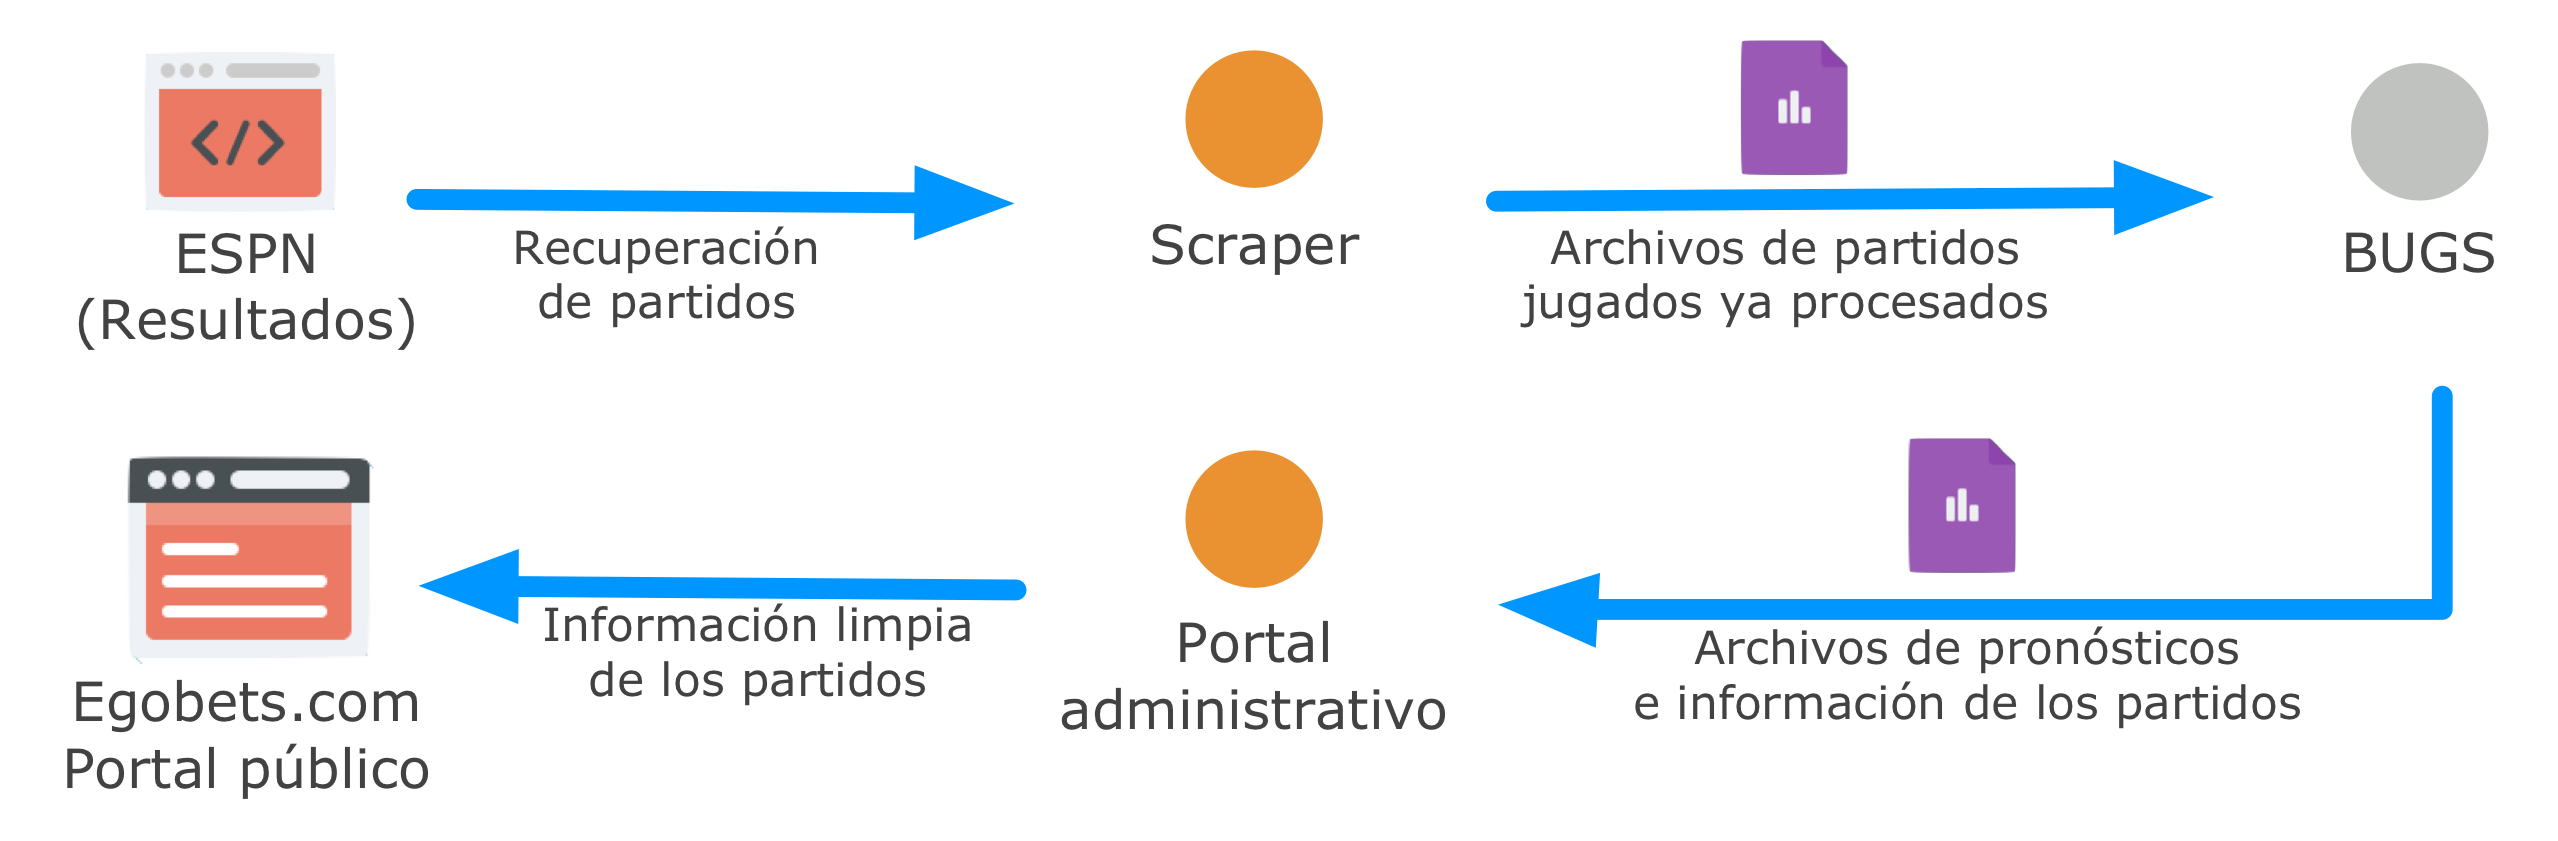
\includegraphics[width=\linewidth]{flujo}
     \caption{Diagrama de flujo de información}\label{Fig:flujo}
   \end{minipage}
\end{figure}

El proceso que se lleva a cabo en el \emph{Back Office} para alimentar el \emph{Portal público} (Ver la figura~\ref{Fig:flujo}), se puede describir de la siguiente manera:
\begin{enumerate}
	\item A través del \emph{Sistema de recopilación} los administradores descargan de la página de Internet de ESPN los resultados de todos los partidos de la temporada junto con la información de los próximos partidos por jugar  de cada una de las ligas Europeas.
	\item Los datos recopilados permiten a los administradores generar un conjunto de archivos de texto con toda la información de los resultados de los últimos partidos y las fechas de los próximos partidos.
	\item Los administradores usan estos archivos para alimentar el \emph{Sistema de estimación} y calcular los pronósticos de los próximos partidos y las probabilidades de los resultados.
	\item Se obtienen los archivos que contienen la información de los próximos partidos así como la información de los equipos por liga y su desempeño en la temporada en curso.
	\item En el \emph{Portal administrativo} se ingestan los archivos obtenidos con la información de los próximos partidos, resultados de partidos anteriores y las estadísticas de los equipos en la temporada en curso.
	\item Finalmente, con la nueva información ingresada, los usuarios podrán disfrutar en el \emph{Portal público} sus recomendaciones peronalizadas de apuestas.
\end{enumerate}


\subsection{Sistema de recopilación de información y estadísticas de los partidos}
\graphicspath{{/Users/brunomedina/Dropbox/Tesis-Egobets/egobets-notas/resources/recopilador/}}
Se desarrolló un sistema web que recupera al principio de cada temporada todos los partidos que se hayan jugado en las temporadas pasadas, así como el calendario de próximos partidos por jugar. Para lograr la extracción de esta información el sistema cuenta con un ``Web Scraper'' que consigue la información de la página de ESPN y la transforma en objetos que después son persistidos en la base de datos. Finalmente, esta información se organiza en un documento CSV para ser descargado por los administradores.

\subsubsection{Tecnologías destacadas}

\begin{itemize}
	\item \textbf{Servidor LAMP.} Esta es una de las configuraciones más populares para servidores web. 
		Una de las principales ventajas de utilizar una arquitectura LAMP es que la mayoría del software utilizado corre bajo la ``Licencia Pública General de GNU'', esta licencia de uso permite a los programadores que utilizan este software, ser capaces de ver el código fuente y en muchos casos le permiten modificarlo y compartirlo \cite{lozano2008software}.
	El famoso acrónimo representa lo siguiente :
	\begin{itemize}
		\item Linux. Sistema operativo Linux (creado por Linus Torvalds), en específico se utiliza la versión de Ubuntu LTS 12.04. Esta versión es estable con una gran comunidad activa de soporte. Algunas de las ventajas de usar Linux son:
		\begin{itemize}
			\item El costo de licencia es gratuito y su uso no tiene algún otro costo monetario.
			\item Hay miles de aplicaciones libres para hacer más robusto el servidor.
			\item Tener las aplicaciones en sus últimas versiones, bien configuradas y aplicar los parches de manera inteligente, garantizan que el servidor se encuentre seguro y sea funcional.
		\end{itemize}
		\item Apache. El servidor HTTP, encargado de recibir y procesar las llamadas HTTP, nació hace diecisiete años como un proyecto por desarrollar un software robusto, de grado comercial, modular y gratuito para servir peticiones (Web) HTTP. Algunas de las ventajas con las que cuenta son \cite{apacheWeb}:
		\begin{itemize}
			\item Gran variedad de módulos. Existen muchos módulos que la comunidad desarrolla para atacar las problemáticas diarias, gracias a que su comunidad es muy activa estos desarrollos nunca acaban.
			\item Fácil de administrar. El soporte de la comunidad y su extensivo uso permite que sea muy sencillo encontrar documentación de como realizar las funciones básicas de administración de servidores como la creación de nuevos dominios, implantación de certificados SSL, etc.
			\item No importa el sistema operativo, Apache corre en UNIX, Windows, Mac y en la gran mayoría de sistemas operativos.
			\item Corre bajo la licencia pública general de GNU.
		\end{itemize}

		\item MySQL. Base de datos relacional que permite al sistema persistir toda la información recuperada del internet. Las principales características de MySQL son \cite{mysqlWeb}:
		\begin{itemize}
			\item Sistema de administración. El servidor MySQL provee las herramientas para agregar, ingresear, procesar y desplegar la información guardada en la base de datos.
			\item Las bases de datos MySQL son relacionales. La información se guarda en tablas separadas en vez de poner todo junto en un solo lugar. Las estructuras de base de datos están organizadas en archivos físicos optimizados para la velcidad. El modelo lógico con objetos como bases de datos, tablas, vistas, tuplas y columnas ofrece un ambiente de programación flexible. Y MySQL se asegura de que se respeten los tipos de relaciones entre tablas como puede ser uno a uno, uno a varios, únicas, u opcionales. Una base de datos bien diseñada nunca permitirá información incosistente, duplicada, huerfana, fuera de fecha o perdida.
			\item Corre bajo la licencia Pública General de GNU. Por lo que se puede modificar y ser utilizado por cualquiera.
		\end{itemize}
				\item PHP: Hypertext Preprocessor.. Según su página Web \cite{phpWeb} es un lenguaje de scripting, el cual puede ser embebido dentro de páginas HTML. Gran parte de su sintaxis fue tomada de C, Java y Perl con un par de características específicas propias de PHP. El objetivo del lenguaje es permitir a desarrolladores Web escribir páginas generadas dinámicamente con agilidad.
				 PHP está enfocado principalmente a la programación de scripts del lado del servidor, por lo que se puede hacer cualquier cosa como recopilar datos de formularios, generar páginas con contenidos dinámicos, o enviar y recibir cookies. Aunque PHP puede hacer mucho más.
				 Ventajas:
		 		\begin{itemize}
		 			\item No depende del sistema operativo. Esto se debe a que corre al ser llamado por el servidor web y PHP corre sobre la mayoría de Servidores web, incluyendo Apache, IIS, lighthttpd, nginx y muchos otros.
					\item No se limita a genera HTML. Puede crear por ejemplo: imágenes, ficheros PDF e incluso películas Flash al vuelo. También puede generar archivos de texto y guardarlos en el sistema de archiso del sistema operativo. 
					\item Permite la conexión casi cualquier Base de datos como: MySQL, SQLite, PostgreSQL, Mongo, Mssql, IBM DB2, entre muchas otras.
					\item PHP también cuenta con soporte para comunicarse con otros servicios usando protocolos tales como LDAP, IMAP, SNMP, NNTP, POP3, HTTP, COM (en Windows) y muchos otros.
					\item Existen muchas otras extensiones interesantes, las cuales están categorizadas alfabéticamente y por categoría.
		 			\item Corre bajo la licencia Pública General de GNU. Por lo que se puede modificar y ser utilizado por cualquiera.
		 		\end{itemize}

	\end{itemize}

	
	\item Code Igniter. Es un framework\footnote{Es una estructura de software compuesta de componentes personalizables e intercambiables para el desarrollo de una aplicación. En otras palabras, un framework se puede considerar como
una aplicación genérica incompleta y configurable a la que se le puede añadir las últimas piezas para construir una aplicación concreta.} de PHP que ahorra tiempo en le programación, robustece tu sistema y permite al programador alcanzar un grado mayor de sofisticación en su código. Uno de los puntos interesantes de este framework es que utiliza el patrón de diseño conocido como Modelo Vista Controlador (MVC), este patrón fue descrito por el noruego Trygve Reenskaug en 1979. 
	Sobre el libro de Upton \cite{upton2007codeigniter} se tiene una aproximación a este patrón de diseño en CodeIgniter:
	\begin{itemize}
		\item Modelos, son objetos que representan los datos. Estos objetos reflejan las tabla de la base de datos y pueden modificarla conforme sea requerido. Los modelos también realizan operacioens a los datos según sea necesario.
		\item Vistas, reflejan el estado del modelo. Son las responsables de desplegar la información al usuario final. En este caso específico, todas las vistas son representaciones HTML del contenido.
		\item Controladores, ofrecen opciones para cambiar el estado del modelo. Son los encargados de consultar los modelos. Proveen a las vistas los datos dinámicos a mostrar.
	\end{itemize}
	De su página Web \cite{codeigniterWeb} se pueden destacar las siguientes propiedades:
	\begin{itemize}
		\item Tamaño pequeño. CodeIgniter 2.2 tiene una descarga 2.2MB, incluyendo la guía del usuario.
		\item Documentación clara. La guía que se incluye cuenta con guía y tutoriales para empezar a trabajar de manera muy práctica.
		\item Compatibildad con casi cualquier servicio de alojamiento. Sólo necesita PHP 5.1.6 y tiene soporte con las bases de datos más comunes incluído MySQL.
		
		\item Casi no necesita configuración. Todas las variables y opciones de configuración vienen predefinidas a los estandares convenidos en internet.
		
	\end{itemize}
	
	
	\item PHP Simple HTML DOM Parser
	Es un script de PHP que permite interpretar el HTML DOM de una página web y permite manipularlo de manera muy sencilla. Requiere PHP 5 o mayor, soporta archivos HTML mal formados y permite encontrar las etiquetas HTML con selectores como lo haría jQuery. Con una simple línea de código basta para extraer los contenidos de una página HTML \cite{htmlparserWeb}.
	\cite{chen2009php} \cite{chowdhury2014intelwiki}
	\item Bootstrap. Es un framework elegante, intuitivo y poderoso que agiliza y facilita el desarrollo Web de front-end Su principal objetivo es facilitar el desarrollo de sitios móviles y responsive. 
	Documentación amplia y detallada, docenas de elementos HTML, componentes CSS e increíbles plugins de jQuery son algunas de sus principales características\cite{bootstrapWeb}. 
	\cite{otto2010bootstrap}
	\cite{cochran2012twitter}
	
\end{itemize}

\subsubsection{Web Scraper}
El proceso de ``Web Scraping'' consiste en extraer y crear representaciones estructuradas con la información de un sitio Web en particular. HTML, el lenguaje de marcado usado para darle estructura a la información de las páginas web está sujeta a muchos cambios, especialmente cuando se actualiza su estilo. Ya que las técnicas de extracción se basan en el lenguaje de marcado, un solo cambio puede llevar a extraer datos incorrectos o incompletos \cite{cording2011algorithms}.

Las técnicas de ``Web Scraping'' permiten, por ejemplo, que una compañía monitoree los precios de los productos de sus competidores. De igual manera le permiten a Egobets, conseguir la última información detallada con la información de las fechas de los partidos, marcadores, tiros a gol, posesión del balón y nombres de los equipos.

Si el dueño de la información no provee de una API abierta, el remedio (como en el caso de Egobets) es el de escribir un programa que apunte a la información desplegada en la página Web. Las propiedades buscadas en un scraper son:
\begin{itemize}
	\item Ser tan tolerante como pueda ser posible a cambios en el lenguaje de marcado.
	\item Ser lo suficientemente rápido como para ofrecer respuestas en milisegundos y evitar ``time-outs'' durante el consumo del servicio.
	\item No tener restricciones en los patrones que conforman la estructura del HTML del sitio. En específico esto implica que el servicio debe ser lo suficientemente bueno como para interpretar de la mejor manera la información aún incluso si el HTML se encuentra mal formado
\end{itemize}

Cording, P. \cite{cording2011algorithms} presenta en su tesis de maestría un estudio de como realizar un scraper que base su funcionamiento en la coincidencia aproximada de los patrones de un árbol, esta es la base de muchas de las librerías que existen (incluyendo la que se usa en este trabajo). Para realizar esta tarea se utiliza una librería de código abierto que permite manipular DOM\footnote{W3schools \cite{domWeb} lo define como: ``Documento W3C Object Model (DOM) es una interfaz de la plataforma y de lenguaje neutro que permite a los programas y scripts acceder y actualizar dinámicamente el contenido, la estructura y el estilo de un documento.''} de HTML y conseguir la información necesaria, esta libreria se llama: PHP Simple HTML DOM Parser. 

\textbf{Un ejemplo de uso}

Supóngase el siguiente HTML:

\lstset{language=HTML}
\begin{lstlisting}[frame=single]
<div class="team-names">
	<div class="team-name">
		<span>
			<img src="http://espncdn.com/teamlogos/soccer/500/102.png" alt="Villarreal" width="22">
			Villarreal
		</span>
	</div>
	<div class="team-name">
		<span>
			<img src="http://espncdn.com/teamlogos/soccer/500/93.png" alt="Athletic Bilbao" width="22">
			Athletic Bilbao
		</span>
	</div>
</div>
\end{lstlisting}

Ahora analícese el siguiente código:

\lstset{language=PHP}
\begin{lstlisting}[frame=single]
	$aux = $table->find('.team-name',0);
	$nomEquipoLocal = $aux;
	$partido['prints']['local_nom']= $nomEquipoLocal;
	$idEspnEquipoLocal = trim(strstr(substr(strstr($aux->innertext, 'soccer/500/'), strlen('soccer/500/')),'.png',true));
\end{lstlisting}


Con este código se pueden obtener los nombres del equipo local y el identificador que le asigna ESPN a sus equipos. Esto es gracias a que \emph{``find('.team-name',0)''} recorre todo el árbol DOM y encuentra todas las ocurrencias de la clase con nombre \emph{``team-name''} el cero que se le proporciona a la función \emph{find} regresa el primer elemento encontrado. De ahí, la propiedad \emph{``->innertext''} muestra la cadena de caracteres plana que contiene ese elemento, por lo que basta con hacer un manejo de cadenas de caracteres para obtener el identificador del equipo que se nombra el archivo PNG del logo del equipo. Para más ejemplos y documentación de como utilizar la librería dirigirse a \cite{sourceparserWeb}.
% Es un script que
% \cite{hogue2005thresher}
% Definir lo que es un scraper
%
%
% Definir las páginas que se buscan y como se recorren
%
% Definir los objetos finales de la base de datos que se consumen.
%
%


\subsubsection{Descripción de su funcionamiento}

\begin{enumerate}
	\item \textbf{Equipos de la temporada.}
	Para poder comenzar la recuperación de información, es importante contar con los equipos que estén jugando esta temporada. Dependiendo de los resultados de la temporada anterior, los equipos que hayan quedado hasta abajo en la tabla de posición descienden a ligas menores y a su vez suben los mejores de estas ligas. Ver figura~\ref{Fig:los-equipos}
	\begin{figure}[!htb]\centering
	   \begin {minipage}{1\textwidth}
	     \frame{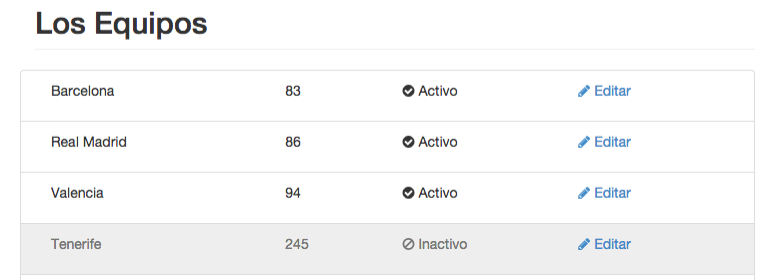
\includegraphics[width=\linewidth]{los-equipos}}
	     \caption[Ejemplo de equipos de la liga española]{Ejemplo de equipos de la liga española\footnotemark }\label{Fig:los-equipos}
	   \end{minipage}
	\end{figure}

	
	\item \textbf{Calendario de próximos partidos.}
	\begin{figure}[!htb]\centering
	   \begin {minipage}{1\textwidth}
	     \frame{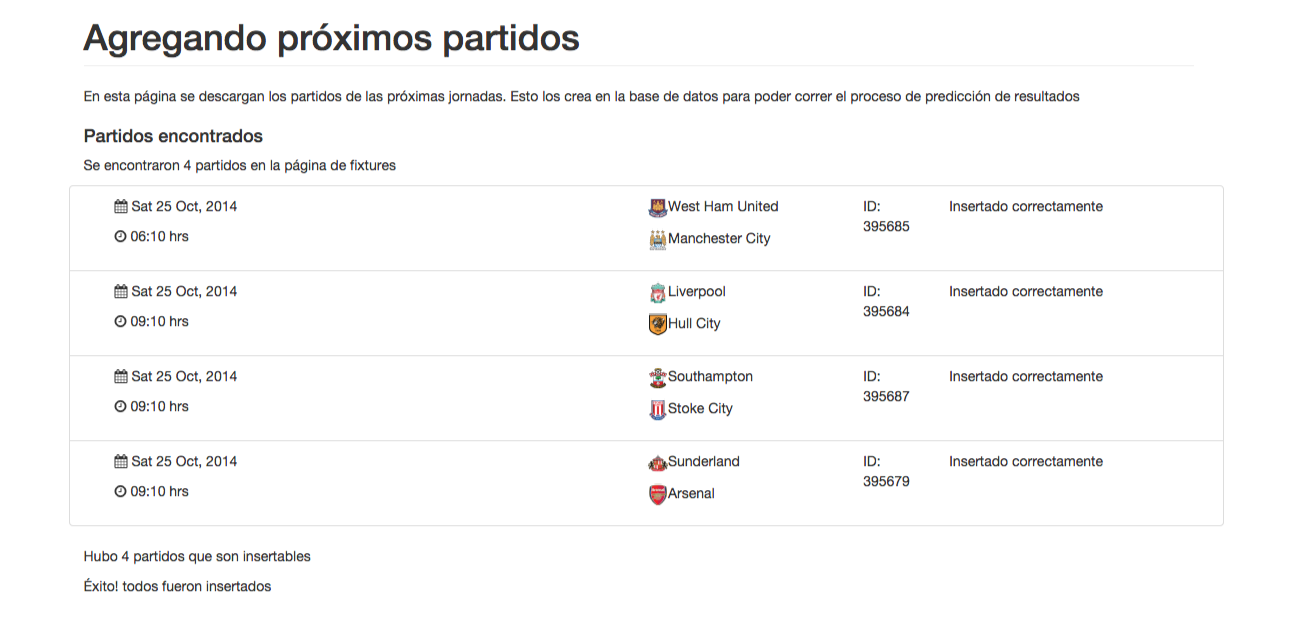
\includegraphics[width=\linewidth]{proximos-partidos}}
	     \caption{Recuperación de próximos partidos}\label{Fig:proximos-partidos}
	   \end{minipage}
	\end{figure}
	
	\item \textbf{Estadísticas e información de partidos jugados.}
	\begin{figure}[!htb]\centering
	   \begin {minipage}{1\textwidth}
	     \frame{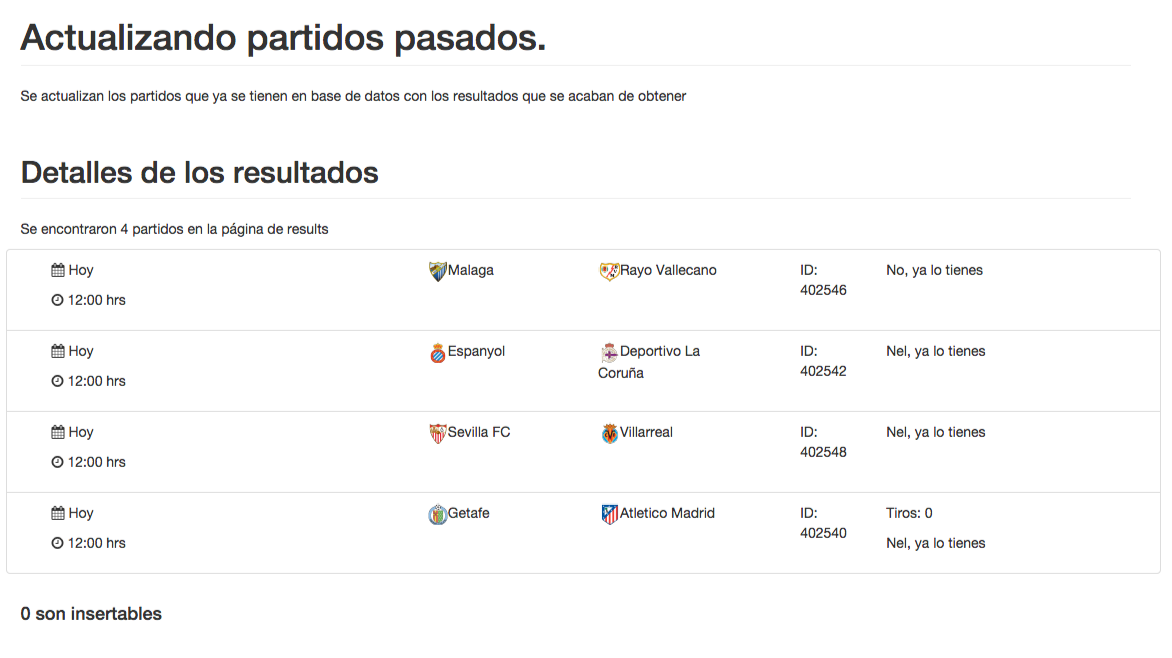
\includegraphics[width=\linewidth]{pasados-partidos}}
	     \caption{Recuperación de resultados de partidos ya jugados}\label{Fig:pasados-partidos}
	   \end{minipage}
	\end{figure}
	\item \textbf{Generación de archivos con resultados.}
	Es importante mencionar que se usan aproximadamente los últimos quinientos partidos para la generación de los archivos, esto implica que se deben tener en base de datos los equipos que participaron en las pasadas dos temporadas de juegos. Por este motivo de pueden encontrar equipos que se encuentran en el sistema con la bandera de inactivos.
	
\end{enumerate}













\subsection{Sistema de estimación de probabilidades}
Adicionalmente en esta sección se describirá el funcionamiento del Sistema de Estimación. Sin embargo, al ser un conjunto de programas en \emph{Fortran} que son ajenos al autor, no se profundizará en los detalles del desarrollo del mismo. Sin embargo, se dará la pauta para entender como se podrían generar probabilidades y pronósticos de los partidos.

\subsubsection{Predicciones}



\cite{rue2000prediction}

\cite{baio2010bayesian}

\cite{dixon2004value}

\cite{koopman2013dynamic}

 \subsubsection{Tecnologías destacadas}

\begin{itemize}
	\item \textbf{Fortran}
	\cite{robison1996c++}
	\cite{veldhuizen1997will}
\end{itemize}
	
\subsubsection{Descripción de su funcionamiento}

Montecarlo
Poisson
Nonormal
Markov


\subsection{Portal administrativo}

\subsubsection{Sitio web para los administradores}

 \cite{alfredo2005ingenieria}
 
 \subsubsection{Tecnologías destacadas}
 
 \begin{itemize}
 	\item LNNP
 	\item Code Igniter
 	\item Raphael
 \end{itemize}
 
 \subsubsection{Diagrama de base de datos}
 
 \subsubsection{Descripciónde su funcionamiento}
 
 \begin{itemize}
 	\item CRUD
 	\item Ingesta de archivos
	
 \end{itemize}
 

\section{Portal público Egobets.com}

\subsection{Características principales}
\subsubsection{Sitio web para los jugadores}
\subsubsection{Tecnologías destacadas}
 
 \begin{itemize}
 	\item LNNP
 	\item Code Igniter
 	\item Parallax
 \end{itemize}
  
\subsubsection{Módulos}

 \begin{itemize}
 	\item Tablero
 	\item Mis Equipos
 	\item Ligas
 	\item Partidos
 	\item Perfil
 	\item Pagos
 	\item Perfil de riesgo
 	\item Sistemas de reserva
 \end{itemize}
 
 \subsection{Proceso para la selección de apuestas}

% Uno de los conceptos más imporantes en la teoría de probabilidad es el del valor esperado de una variable aleatoria\footnote{Retómese el concepto de variable aleatoria más usual, se puede utilizar la definición del capítulo 4 del libro de Ross \cite{ross2006first}, una función $X$ que genera valores aleatorios reales en un espacio muestral completamente definido.}, en palabras del señor Ross \cite{ross2006first} el valor esperado de $X$ se define como un promedio ponderado de los valores posibles que puede tomar $X$; se pondera cada valor con la probabilidad de que $X$ tome ese preciso valor.
%  \begin{itemize}
%
%  	\item Valor esperado de una variable discreta.
%
% 		\[E[X] = \sum_{x:p(x)>0}x p(x)\]
%  	\item Valor esperado de una variable continua.
% 	\[E[X] = \int_{-\infty}^{infty} f(x) dx\]	
 % \end{itemize}
 
 El proceso de la recomendación de apuestas se puede dividir en cinco pasos principales:

 \begin{enumerate}
 	\item \textbf{Determinación de apuestas redituables.} De todas las apuestas de las cinco ligas que haya en la jornada a recomendar, se escogen únicamente aquellas que sean redituables a largo plazo. Independientemente del nivel de riesgo de cada cliente, se generarán recomendaciones únicamente de apuestas que, al analizarlas, tengan ganancias esperadas.
 	\item \textbf{Selección de apuestas de acuerdo al riesgo del cliente.} Las estimaciones de cada partido tienen un intervalo de confianza. Con base en este intervalo y el perfil de riesgo del usuario se seleccionan las apuestas.
 	\item \textbf{Cálculo de la proporción del dinero a invertir por apuesta.} Al conocer la selección de las apuestas, se calcula la proporción de dinero a invertir para cada apuesta, este proceso sigue siendo dependiente de la confianza de la estimación del partido y de la adversidad al riesgo del cliente.
 	\item \textbf{Determinación del nivel de reservas.} En este paso se cuenta con un conjunto seleccionado de apuestas y la proporción de dinero que se debe invertir para cada una de ellas. Acorde a su encuesta, se calcula el nivel óptimo de reservas que le permitan al cliente seguir apostando a pesar de que tenga una mala jornada y pierda todas las apuestas.
 	\item \textbf{Recomendación.} Todos estos elementos constituyen en su totalidad la recomendación de la semana que se presenta en el portal al cliente.
 \end{enumerate}
 
Para definir el escenario completo es necesario definir las variables que se utilizan en el proceso, así como las funciones de utilidad que modelan los perfiles de riesgo de los usuarios. Después de estas dos subsecciones se retomará paso a paso la explicación del proceso de recomendación de apuestas.
 
\subsubsection{Variables necesarias}

En este apartado de la tesis se explica cómo se determinan los partidos que se recomiendan a los clientes.
Las variables que se necesitan utilzar son las siguientes:
\begin{enumerate}
	\item \textbf{Probabilidades.} Ya en apartados anteriores se habló de las probabilidades estimadas de que ocurran los tres diferentes resultados de cada encuentro de la jornada (Victoria del local, del visitante y empate). Estas probabilidades son alimentadas a través del portal administrativo.
	
	\item \textbf{Momios.} Los momios que generan las casas de apuestas para cada partido. En la mayoría de los escenarios el usuario escoge usar todos los momios de todos los bookies, en estos casos se tomarán los momios que ofrezcan mejores retornos para cada partido. Estos momios se toman de la información pública de las casas de apuestas.
	
	\item \textbf{Variables de riesgo.} Se tienen tres elementos principales que generan la noción de riesgo en el sistema:
	\begin{itemize}
		\item \textbf{Función de utilidad en selección.} Determina los partidos redituables de la jornada.
		\item \textbf{Función de utilidad del dinero.} Dicta la proporción de dinero a apostar en cada partido.
		\item \textbf{Variable de reserva.} Marca la cantidad de dinero que el cliente debería guardar para siguientes apuestas.
		Estas variables dependen de la encuesta que se le presenta al cliente al crear su cuenta.
	\end{itemize}
	
	\item \textbf{Variable de evolución de ingreso del cliente.} Se define como la cantidad de dinero que tiene el cliente en esta jornada entre la máxima cantidad de dinero que ha tenido. Esta variable genera una noción, en caso de que existan, de la magnitud de las pérdidas que ha tenido el cliente.
\end{enumerate}

\subsubsection{Funciones de utilidad}
Para modelar el comportamiento de un individuo ante el riesgo, se utilizan funciones de utilidad. Estas funciones representan la utilidad (o beneficio) que un individuo puede obtener por una apuesta. Las funciones más arriesgadas le dan valores mayores valores a las apuestas que que ofrecen las mejores ganancias y las funciones más conservadoras favorecen aquellas apuestas con mayores probabilidades.
En particular, se podría decir de manera intuitiva que el valor obtenido por una función de utilidad para una apuesta en particular es la cantidad de unidades de dinero que el individuo estaría dispuesto a invertir en esa apuesta.
El siguiente listado presenta las funciones que se utilizan actualmente en el sistema.
\begin{enumerate}
		\item \textbf{Polinomial - lineal:} 
		\[f_1(\alpha, p, m) = \left(\frac{p}{1-p} \right)^\frac{1}{1-\alpha}(m-1)^\frac{\alpha}{1-\alpha}\]
Parámetro $\alpha$ que va de cero a uno. Es una de las familias más volatiles en cuanto al riesgo, para valores cercanos a uno del parámetro tiende a ser muy arriesgada, casi sin diversificar, y para valores cercanos a cero tiende a ser muy conservadora y suele diversificar mucho más en las apuestas.

		\item \textbf{Polinomial - cuadrática:} 
		\[f_2(\alpha, p, m) = \left(\frac{p}{1-p} \right)^\frac{1}{2-\alpha}(m-1)^\frac{\alpha}{2-\alpha}\]
Esta familia de funciones es muy parecida a la anterior, también tiene un parámetro $\alpha$ entre cero y uno, sólo que en este caso no es tan extremista como en el caso anterior.
		
		\item \textbf{Exponencial - lineal:} 
		\[f_3(\alpha, p, m) = \left(\frac{1}{m-1} \right)ln\left(\frac{\alpha p(m-1)}{1-p}\right)\]
Esta familia de funciones tiene un parámetro $\alpha$ que es mayor a uno. Es una familia de funciones conservadoras que suelen proteger muy bien adelatandose a semanas malas, a costo que en semanas buenas no logran tan buenos beneficios.
		
		\item \textbf{Lineal - exponencial:} 
		\[f_4(\alpha, p, m) = ln\left(\frac{p(m-1)}{1-p}\right) + ln(\alpha)\]
Esta familia de funciones tiene un parámetro $\alpha$ que es mayor a uno. Es una familia de funciones que le gusta fuertemente diversificar, aparte tiende a favorecer un poco aquellas apuestas más riesgosas.

		\item \textbf{Logarítmica - polinomial:} 
		\[f_5(\alpha, p) = \left(\frac{p}{1-p}\right)^\frac{1}{\alpha}\]
Parámetro $\alpha$ mayor a uno. Es una familia de funciones muy conservadora ya que toma valores sin considerar los momios del mercado, al tomar en cuenta solamente las probabilidades de los partidos tiende a ser más estable en el tiempo.

		\item \textbf{Tangente - lineal:} 
		\[f_6(\alpha, p, m) = \frac{1}{m-1}\sqrt{\frac{pm - (1-\alpha)p - \alpha}{1-p}}\]
		Parámetro $\alpha$ entre cero y uno. Esta familia es la más conservadora de la lista, busca tener las menores pérdidad posibles y protege las inversiones cada semana.
\end{enumerate}

Estas seis funciones son las que utiliza Egobets para modelar la adversidad al riesgo de sus clientes. Cuando ellos llenan la encuesta del perfil, realmente están seleccionando una de estas funciones.


\subsubsection{Paso 1 - Determinación de apuestas redituables}
\label{sec:paso-1}


Para seguir la explicación de los pasos del proceso se tomará un ejemplo práctico y las transformaciones que sufre durante el proceso. Al empezar las recomendaciones de una jornada se tiene un conjunto de datos muy parecido al que se da en el ejemplo. Tómese la tabla~\ref{momios-y-probas} como base del ejemplo. En esta tabla se presentan momios de alguna casa de apuesta (usualemente los mejores del mercado) para diez partidos distintos, cada uno cuenta con los momios para los tres tipos de apuestas: victoria del Local ($m_L$), empate ($m_E$) y victoria del visitante ($m_V$). Además se muestran las probabilidades estimadas por Egobets de los tres posibles resultados del encuentro: victoria del local ($\hat{p_L}$), empate ($\hat{p_L}$) y victoria del visitante ($\hat{p_L}$).

\begin{table}[h]
\centering
\resizebox{\textwidth}{!}{%
\begin{tabular}{|c|ccc|ccc|}
\toprule
{\textbf{Partido}}                 & $\mathbf{m_L}$ & $\mathbf{m_E}$ & $\mathbf{m_V}$ & $\mathbf{\hat{p_L}}$ & $\mathbf{\hat{p_E}}$ & $\mathbf{\hat{p_V}}$ \\ \midrule
A & 2.6  & 3.2  & 2.75  & 0.31  & 0.23  & 0.46  \\ 
B & 2.1  & 3.3  & 3.5   & 0.37  & 0.3   & 0.32  \\ 
C & 1.11 & 8.5  & 21    & 0.84  & 0.1   & 0.04  \\ 
D & 4.5  & 3.75 & 1.72  & 0.29  & 0.27  & 0.45  \\ 
E & 2    & 3.4  & 3.75  & 0.37  & 0.31  & 0.31  \\ 
F & 1.53 & 4    & 6     & 0.61  & 0.17  & 0.21  \\ 
G & 2.1  & 3.25 & 3.6   & 0.51  & 0.24  & 0.25  \\ 
H & 1.9  & 3.4  & 4     & 0.42  & 0.29  & 0.29  \\ 
I & 1.8  & 3.5  & 4.5   & 0.46  & 0.29  & 0.25  \\ 
J & 1.9  & 3.4  & 4     & 0.5   & 0.26  & 0.23  \\ \bottomrule
\end{tabular}
}
\caption{Diez partidos con sus respectivos momios y las probabilidades estimadas por Egobets}
\label{momios-y-probas}
\end{table}

Para concretar el ejemplo, se fijarán las siguientes funciones y variables.
\begin{itemize}
	\item \textbf{Funcion de selección.} Tómese la \emph{Polinomial - lineal} $f_1$ con parametro $\alpha = 0.4$.
	\item \textbf{Funcion de utilidad del dinero.} Úsese la \emph{Exponencial - lineal} con parámetro $\alpha = 3$
	\item \textbf{Variable de reserva.} Será $v_R = 15$.
	\item \textbf{Variable de ingreso.} Será $v_I = 0.80$.
\end{itemize}
	

Ahora para proceder al primer paso, defínase el valor esperado de una apuesta como la multiplicación de la probabilidad de que suceda el resultado por el momio que se tiene para esa apuesta. 
Con el ejemplo bien definido se procede a filtrar las apuestas con el primer paso. De manera intuitiva, se podría enunciar que el valor esperado de una apuesta corresponde a la cantidad de unidades de dinero que se obtienen por cada unidad de dinero invertida\footnote{Recuérdese que esta cantidad incluye la cantidad de dinero invertida en la apuesta. También recuérdese que la ganancia solamente se obtiene si se gana la apuesta.}

Entonces, el primer paso consiste en utilizar para las recomendaciones, sólo las apuestas con ganancias a largo plazo; las otras apuestas tendrán un valor esperado no positivo, es decir, no garantizan más que pérdidas a largo plazo. Más aun, se usarán solo las apuestas que garanticen un valor esperado mayor a $1.025$, esta restricción tiene dos ventajas, la primera es que las probabilidades que se usan son estimaciones por lo que ese $2.5\%$ funciona como protección para no caer en valores esperados negativos y la segunda es que si el rendimiento es tan pequeño toma mucho tiempo para un cliente ir acumulando ganacias. 

\begin{table}[ht]
\centering
\resizebox{\textwidth}{!}{%
\begin{tabular}{|c|ccc|ccc|ccc|c|}
\toprule
Partido & $\mathbf{m_L}$ & $\mathbf{m_E}$ & $\mathbf{m_V}$ & $\mathbf{\hat{p_L}}$ & $\mathbf{\hat{p_E}}$ & $\mathbf{\hat{p_V}}$ & $\mathbf{m_L\cdot\hat{p_V}}$ & $\mathbf{m_E\cdot\hat{p_E}}$ & $\mathbf{m_V\cdot\hat{p_V}}$ & \textbf{Apuesta} \\ \midrule
A & 2.6 & 3.2 & 2.75 & 0.31 & 0.23 & 0.46 & 0.81 & 0.74 & \textbf{1.27} & Visitante \\
B & 2.1 & 3.3 & 3.5 & 0.37 & 0.3 & 0.32 & 0.78 & 0.99 & \textbf{1.12} & Visitante \\
C & 1.11 & 8.5 & 21 & 0.84 & 0.1 & 0.04 & 0.93 & 0.85 & 0.84 & Ninguna \\
D & 4.5 & 3.75 & 1.72 & 0.29 & 0.27 & 0.45 & \textbf{1.31} & 1.01 & 0.77 & Local \\
E & 2 & 3.4 & 3.75 & 0.37 & 0.31 & 0.31 & 0.74 & \textbf{1.05} & \textbf{1.16} & Empate/Visitante \\
F & 1.53 & 4 & 6 & 0.61 & 0.17 & 0.21 & 0.93 & 0.68 & \textbf{1.26} & Visitante \\
G & 2.1 & 3.25 & 3.6 & 0.51 & 0.24 & 0.25 & \textbf{1.07} & 0.78 & 0.90 & Local \\
H & 1.9 & 3.4 & 4 & 0.42 & 0.29 & 0.29 & 0.80 & 0.99 & \textbf{1.16} & Visitante \\
I & 1.8 & 3.5 & 4.5 & 0.46 & 0.29 & 0.25 & 0.83 & 1.02 & \textbf{1.13} & Visitante \\
J & 1.9 & 3.4 & 4 & 0.5 & 0.26 & 0.23 & 0.95 & 0.88 & 0.92 & Ninguna\\ \bottomrule
\end{tabular}
}
\caption{Escogiendo apuestas que vale la pena realizar}
\label{redituables}
\end{table}

Observese en la tabla~\ref{redituables} como en negritas se han señalado las posibles apuestas a realizar. De las treinta posibles apuestas, ahora sólo quedan 9 redituables. Hay dos partidos el `C' y el `J' que no ameritan apuesta alguna. Y el partido `E', por ejemplo, tiene dos posibles apuestas redituables.

\subsubsection{Paso 2 - Selección de apuestas}
\label{sec:paso-2}


Para determinar el portafolio de apuestas basta con calcular el valor de la función de utilidad de selección y se deben tomar aquellas ``$n$'' apuestas que tengan los mayores valores (Donde ``$n$'' es el número de apuestas a recomendar).
Ver tabla~\ref{seleccion}

\begin{table}[ht]
\centering
\resizebox{\textwidth}{!}{%
\begin{tabular}{|c|c|c|c|c|}
\toprule
\textbf{Partido} & \textbf{Apuesta} & \textbf{Momio} & $\mathbf{\hat{p}}$ & $\mathbf{f_1(\alpha, p, m)}$ \\ \midrule
A & Visitante & 2.75 & 0.46 & \textbf{1.07} \\
B & Visitante & 3.5 & 0.32 & 0.53 \\
D & Local & 4.5 & 0.29 & 0.49 \\
E & Empate & 3.4 & 0.31 & 0.48 \\
E & Visitante & 3.75 & 0.31 & 0.53 \\
F & Visitante & 6 & 0.21 & 0.31 \\
G & Local & 2.1 & 0.51 & \textbf{1.12} \\
H & Visitante & 4 & 0.29 & 0.48 \\
I & Visitante & 4.5 & 0.25 & 0.36\\ \bottomrule
\end{tabular}
}
\caption{Escogiendo apuestas que vale la pena realizar}
\label{seleccion}
\end{table}

\subsubsection{Paso 3 - Calcular cuanto dinero a cada apuesta}
\label{sec:paso-3}

Una vez determinado el portafolio de apuestas hace falta determinar la cantidad de dinero que se invertirá en éste. Esta sección y la próxima resolverán tal problema.
 Empezamos por determinar cuál es la proporción de dinero que se invertirá en cada apuesta. La solución es sencilla, ya determinamos en secciones anteriores que el valor definido por una función de utilidad puede ser comparado con la cantidad de unidades de dinero que una persona estaría dispuesta a invertir en una apuesta en particular. El único problema con este enfoque es que tales cantidades no se encuentran en ninguna escala (es decir, dolares, pesos, etc).Lo que hacemos es lo siguiente: para cada apuesta calculamos el valor de su funcion de utilidad del dinero y después lo dividimos entre la suma de todos estos valores para todas las apuestas que se van a tomar, de esta forma tenemos los números como porcentajes.
 Regresando al ejemplo: (En este caso la función de utilidad del dinero era Exponencial-Lineal con parámetro 3)
Ver tabla~\ref{proporcion}

\begin{table}[ht]
\centering
\resizebox{\textwidth}{!}{%
\begin{tabular}{|c|c|c|c|c|}
\toprule
\textbf{Partido} & \textbf{Apuesta} & \textbf{Momio} & $\mathbf{\hat{p}}$ & $\mathbf{f_3(\alpha, p, m)}$ \\ \midrule
A & Visitante & 2.75 & 0.46 & 0.23 \\
G & Local & 2.1 & 0.51 & 0.35 \\ \bottomrule
\end{tabular}
}
\caption{Calculando la proporción del dinero que se debe invertir en estas apuestas}
\label{proporcion}
\end{table}


Los valores suman a 0.59, cuando se divide cada valor por 0.59 resulta: De la cantidad a apostar, se debe de apostar $40 \%$ en el partido A a visitante y $60 \%$ en el partido G a local.


\subsubsection{Paso 4 - Determinar nivel de reservas}
\label{sec:paso-4}

%[COMENTARIO]ESto no creo que vaya aquí, estas propiedades deberían estar definidas en otro lugar
% El sistema de reservas, en pocas palabras, tiene como intención proteger el dinero de los clientes en el corto plazo, de tal forma que si una semana resulta en pérdidas, éstas no vayan a afectar la tendencia a largo plazo de sus ingresos totales. Las ventajas de usar un sistema de reservas son las siguientes: primero, como ya se dijo, proteger el dinero del cliente en el corto plazo cuando haya pérdidas, en segundo lugar, permite al cliente mantener el mismo nivel de apuestas cada semana, y tercero, permite darle una estructura de fondo de inversión a las apuestas y así poder aprovechar el potencial interés compuesto que resulte de apostar. En contraste, las desventajas son: en cada semana se decide apostar menos dinero y por lo tanto las ganancias son menores en el corto plazo, además al ser una estrategia de largo plazo, los clientes que deseén incurrir en mayores riesgos no usarán este sistema de reservas.
%
% Un sistema de reservas da más flexibilidad de la que inicialmente se podría pensar, estas son algunas de las propiedades que serían deseables en un sistema de esta forma:
% \begin{enumerate}
% \item Se tenga la seguridad de que con alta probabilidad el apostador nunca va a perder todo su dinero.
%
% \item Que en aquellas semanas que son mas riesgosas se apueste menos dinero, para protegerse del riesgo.
%
% \item Que en aquellas semanas donde se pueden tener muchas ganancias se apueste una mayor cantidad de dinero, para tratar de aprovechar situaciones ventajosas.
%
% \item Que cuando se tengan pérdidas se apueste una mayor cantidad de dinero para tratar de recuperar el nivel anterior de ganancias lo más pronto posible.
% \end{enumerate}
% Como se ve, este sistema tiene la propiedad de ser dinámico y que depende tanto de las circunstancias de las apuestas como también del historial de ganancias del cliente.

Determinar el nivel de reservas es un algoritmo que depende del historial de ganancias del cliente así como de las circunstancias de las apuestas que se le presentan al cliente. A continuación se explica paso a paso como determinar el nivel de reservas.

\begin{enumerate}
	\item \textbf{Calcular la cantidad de partidos a los que se apuesta.}
	
	
Defínase $j$,$k$ como la cantidad de partidos a apostar y el número de apuestas a tomar, respectivamente.
En este pasó bastará con calcular $j$. Sin embargo, es importante notar que hay veces en las que puede haber más de una apuesta sugerida para un mismo partido, i.e. $k>j$. En estos casos se deberá ser cuidadoso de no contar doble los partidos que ya tengan apuestas.

	% Sea $k$ el numero de a
	% \lstset{language=Pascal}
	% \begin{lstlisting}[frame=single]
	% begin
	% 	apuestas := 0;
	% 	aux2 := 0;
	% 	for i:= 1 to K do
	% 	begin
	% 		if (proporcion(i) >= 1/k) then
	% 			aux1 := aux1 + 1;
	% 		else
	% 			aux2 := aux2 + proporcion(i);
	% 	end;
	% 	partidosApostables := aux1 + round((k)aux2);
	% end.
	% \end{lstlisting}
	%
	\item \textbf{Calcular el valor esperado y varianza del portafolio de apuesta.}
	
	
	Sean $m_i$, $p_i$ y $prop_i$; el momio, la probabilidad y la proporción de dinero a apostar del partido $i$ respectivamente. Entonces el valor esperado de la apuesta sería:
	\[\mu = \sum_{i=1}^{k}{(prop_i)(m_i)(p_i)}\]
	Y el riesgo o varianza del portafolio de apuestas se calcula así:
	\[\sigma = \sqrt{\sum_{i=1}^{k}{(prop_i))^2(m_i)^2(p_i)(1-p_i)}}\]
	
	
	\item \textbf{Actualizar el riesgo del portafolio.}
	
	
	Sea $\rho$ el parámetro de reserva un número entereo entre $10$ y $25$ dependiendo de la encuesta del cliente. Se actualiza el riesgo del portafolio al multiplicarlo por un escalar proveniente de la raiz cuadrada del cociente de la cantidad de partidos $j$ entre el parámetro de reserva $\rho$.
	\[\sigma = \left(\sqrt{\frac{j}{\rho}}\right)\sigma\]
	

	\item \textbf{Calcular probabilidad de riesgo.}
	
	Sea $X$ la variable de evolución del ingreso del cliente (Esta variable es completamente dependiente de las historia de perdidas y ganancias del cliente). Y sea $p_\sigma$ la probabilidad de riesgo y se calcula de la siguiente manera:
	\[p_\sigma = \frac{1}{1.749615}(I_1 + I_2) - 1.06 + X\]
	Donde $I_1$ es
	\[I_1 = 0.2925 +1.3772\mu - 1.127\rho\]
	e $I_2$ equivale a
	\[I_2 = \frac{3.11}{\mu}(1 + 0.792\sigma - \mu)((-0.567345 + 1.3772\mu -1.17\sigma)\mu X)^{0.123}\]
	
	
	\item \textbf{Calcular variable proxy.}
	
	 Sea $proxy$ la variable auxiliar que tome en cuenta la probabilidad de riesgo en el cálculo.
	 \[proxy = 0.2925 + 1.3772\mu -1.127\sigma - 0.9975p_\sigma\]
	
	\item \textbf{Calcular el nivel de reserva.}
	
	Finalmente, defínase $c_A$ cómo el porcentaje a apostar del ingreso total. El nivel de reserva será uno menos esta proporción.
	
	\begin{equation*}
	    c_A = \begin{cases}
	               0.05            & \text{si } \frac{j(proxy)}{\rho} < 0.05\\
	               1               & \text{si } \frac{j(proxy)}{\rho} >1\\
	              	\frac{j(proxy)}{\rho} & \text{en otro caso}
	           \end{cases}
	\end{equation*}
	
	$C_A$ representa, en porcentaje, la cantidad de dinero que se le recomendará al cliente que apueste en esa semana para el portafolio de apuests en cuestión.
	
	\textbf{Calculando el nivel de reserva en el ejemplo.}
	
	Primero que nada es importante recordar cuanto valían las distintas variables y establecer los valores necesarios para el ejemplo.
	\begin{itemize}
		\item $k = 2$ (Cantidad apuestas a realizar)
		\item $\rho = 15$ (Parámetro de reserva en función de las preferencias del cliente)
		\item $X = 0.80$ (Evolución del ingreso del cliente)		
	\end{itemize}
	Ahora se procederá a calcular el nivel de reservas.
	\begin{enumerate}
		\item Se obtiene $j = 2$ (Cantidad de partidos en los que se apuesta)
		\item Se calcula el valor esperado 
		\[\mu = (0.4)(2.75)(0.46) + (0.6)(2.1)(0.51) = 1.1486\] 
		y el riesgo del portafolio 
		\[\sigma = \sqrt{(0.4)^2(2.75)^2(0.46)(0.54)+(0.6)^2(2.1)^2(0.51)(0.49)} = 0.835\]
		\item Se actualiza el riesgo $\sigma = \left(\sqrt{\frac{2}{15}}\right)0.835 = 0.3$
		\item Se calcula la probabilidad de riesgo
		\[I_1 = 0.2925 +1.3772(1.1486) - 1.127(0.3) = 1.53\]
		\[I_2 = \frac{3.11}{1.1486}(1 + 0.792(0.3) - \mu)((-0.567345 + 1.3772(1.1486)\]
		\[-1.17(0.3))(1.1486)(0.8))^{0.123} = 0.2272\]
		Entonces
		\[p_\sigma = \frac{1}{1.749615}(1.53 + 0.2272) - 1.06 + 0.8 = 0.74\]
		
		\item Se calcula la variable auxiliar $proxy = 0.2925 + 1.3772(1.1486) -1.127(0.3) - 0.9975(0.74) = 0.81$
		
		\item La cantidad a apostar es entonces es igual a $c_A = \frac{2(0.81)}{15} = 0.108$
		Por lo tanto, con esta adversidad al riesgo y con base en el portafolio de apuestas de la tabla~\ref{proporcion}.
		
		\textbf{El nivel de reserva para esta recomendación es del} $\mathbf{89.2\%}$.
	\end{enumerate}
\end{enumerate}

\subsubsection{Paso 5 - Presentando la recomendación}
\label{sec:paso-5}
Ahora, con todos los pasos cumplidos lo único restante es poner las cifras juntas. Se toma la proporción calculada en~\ref{sec:paso-3} y se multiplica por la cantidad a apostar obtenida en~\ref{sec:paso-4}.
Más aún, si el usuario proporciona la cantidad de dinero que tiene disponible, las recomendaciones se pueden expresar en moneda.

Finalmente si para el ejemplo planteado en~\ref{sec:paso-1} se conoce que el usuario tiene $\$10'000.00$ para apostar, la recomendación de apuesta quedaría de la siguiente manera:
\begin{enumerate}
	\item Apueste $\$432$ pesos ($4.32\%$) en el partido A a favor del equipo visitante.
	\item Apueste $\$648$ pesos ($8.48\%$) en el partido G a favor del equipo local.
\end{enumerate}


